\chapter{Anforderungen und Konzept}\label{ch:Anforderungen und Konzept}

[...]. Fundamental für diese Arbeit ist es, bestehende Arbeiten aus Kapitel \ref{ch:Verwandte Arbeiten} auf ihre tatsächliche Fähigkeiten zu vergleichen. Um solche Vergleichswerte zu erhalten, bedarf es eigener Experimente, in welchen Code-Generierungs Anwendungen unter gleichbleibenden Bedienungen gegen bestehende Benchmarks ausgeführt werden. In diesem Kapitel sollen die Anforderungen und ds Konhept an diese Experimente erläutert werden.\todo{Rewrite I think, das greift etwas vor}

\section{Anforderungen}\label{ch:Anforderungen}

Um die Forschungsfrage \rqref{RQ1} zu beantworten, wird ein empirischer Vergleich benötigt. Ein solcher Vergleich lässt sich aus den gegebenen Arbeiten allerdings nur schwer ableiten, da die Rahmenbedienungen für die gegebenen Lösungen und deren Evaluation stets unterschiedlich sind. Wir haben hier bereits festgestellt dass:

\begin{itemize}
    \item LLM Modelle
    \item Hyperparameter
    \item Benchmarks und deren Umgebungen
\end{itemize}

in praktisch jeder Arbeit Unterschiede aufweisen. Insofern bedarf es einen eigenen, kontrollierten Versuchsaufbau, mit dem gewährleistet werden kann, dass diese Faktoren konsistent bleiben. Aus dieser Notwendigkeit soll in diesem Kapitel das Konzept für einen solche Aufbau präsentiert werden.

Am Rande gilt es hier zu erwähnen, dass für die Beantwortung von \rqref{RQ2} kein Versuchsaufbau genutzt wird.

\subsection{Funktionale Anforderungen}\label{ch:Funktionale Anforderungen}

Nun gilt es die Anforderungen an eine solche Anwendung zu spezifizieren, damit wir diese in einer späteren Implementierung nachvollziehen können. Es ergeben sich folgende funktionale Anforderungen:

\textbf{Invarianz}\label{req:FA1} \\ Es muss möglich sein, beliebige Lösungsansätze gegen beliebige Benchmarks zu prüfen (bzw. auszuführen).

\textbf{Konfiguration}\label{req:FA2} \\ Eine einheitliche Schnittstelle existiert, die es ermöglicht Modelle, Hyperparameter sowie Lösungsansätze frei zu konfigurieren.

\textbf{Isolation}\label{req:FA3} \\ Die Ausführung von Lösungsansätzen und Benchmarks muss in isolierten Umgebungen stattfinden.

\textbf{Bewertung}\label{req:FA4} \\ Die Bewertung des generierten Codes eines Lösungsansatzes erfolgt ausschließlich durch den gegebenen Benchmark.\todo{Name finden}

\textbf{Protokollierung}\label{req:FA5} \\ Für einzelne Durchläufe werden alle Parameter, Versionen sowie ausgegebene Dateien protokolliert. 

\todo[inline]{Ist wiederholbarkeit evtl. eine Anforderung? Wie läuft das mit Temperature?}

\todo[inline, color=red]{Evtl. die Namen mit ID's versehen, FA1, FA2 und dann NFA1 usw!}

\subsection{Nicht-funktionale Anforderungen}\label{ch:Nich-Funktionale Anforderungen}

Neben den bereits genannten funktionalen Anforderungen, ergeben sich weiterhin auch Nicht-funktionale Anforderungen:

\begin{enumerate}
    \item Generierter Code muss unabhängig und isoliert von seiner Umgebung laufen können. Das selbe gilt für die Bewertung.
    \item Der laufende Benchmark bewertet die Ergebnisse einer laufenden Code-Generierungsanwendung. Die Bewertung wird einzig und allein vom Benchmark definiert.
    \item Alle Code-Generierungsanwendungen müssen austauschbar sein. Dafür dürfen weder der Benchmark noch andere funktionale Aspekte der Anwendung verändert werden.
    \item Jeder Durchlauf eines Experiments muss vollständig nachvollziehbar sein. Versionen, Modelle und Parameter müssen auch nach Durchführung ersichtlich sein.
\end{enumerate}
\todo[inline]{Auch wie funktionale Anforderungen labeln und mit Obernahmen versehen damit die dann in dre Umsetzung referenziert werden können!}

\subsection{Rahmenbedienungen \& Abgrenzung}\label{ch:Rahmenbedienungen_Abgrenzung}

\todo[inline]{Sind externe Abhängigkeiten oder Rahmenbedingungen (z. B.
Plattformen, Zielgruppen, Datenquellen) eindeutig und nachvollziehbar
dargestellt?}

Neben den formulierten Anforderungen muss der Umfang der Anwendung abgegrenzt werden. Auf Grund des Budgets für diese Arbeit ist es nicht möglich massive Testreihen durchzuführen welche z.B. die Evaluationsmetrken $pass@10$ oder gar $pass@100$ abdecken können. Weiterhin gibt es keinen Benchmark welcher User-Stories als Eingabeartefakte bereit stellt. Daher wird hier klar festgelegt dass ein solcher Benchmark nicht Teil der Anforderungen oder der Konzeption sein kann.

Weiterhin ist im Sinne der Integrität zu erwähnen, dass die zu testenden Lösungsansätze in ihrer internen Logik nicht verändert werden dürfen. Lediglich nicht-Logikbasierte Eingriffe (z.B. eine Modifikation, die das Einstellen aller Hyperparameter innerhalb eines LLMs Zugriff ermöglicht) sind erlaubt, da diese für eine uniforme Durchführbarkeit vonnöten sind. Eine Außnahme gilt in diesem Kontext für die Nutzung von selbst etablierten Verfahren, da die Logik hier grundlegend erst geschaffen werden muss und nicht von aussenstehenden Arbeiten stammt.

Eine weitere Abgrenzung gilt den Zielsprachen des generierten Codes. Dieser kann nicht frei gewählt werden, da er direkt vom Benchmark und dessen Evaluation abhängig ist.
\todo[inline]{Falls SWE-Pro (oder verified?) dann evtl erwähnen dass es hier mehr als Python gibt. Ansonsten einfach sagen dass es halt nur Python ist, nicht mehr. Das könnte man auch am Ende nochmal auffassen, da es hier bereits angesprochen wurde.}

\section{Konzept}\label{ch:Konzept}

In dieser Sektion soll das Konzept des Versuchsaufbaus erläutert werden. 

\subsection{Untersuchungsdesign}\label{ch:Untersuchungsdesign}

Zu Grunde liegt dass Problem der Vergleichbarkeit. Praktisch alle referenzierten Arbeiten hab eine vielzahl an Parametern, mögen diese spezifische Hyperparameter oder globalere Parameter wie Modelle oder sogar Benchmarks sein. Dies macht es fundamental nicht möglich einen klaren Vergleich zu ziehen, denn für diesen dürfte sich wenn möglich nur ein Parameter ändern, nämlich der Lösungsansatz zur Code-Generierung.

Aus diesem Grund verläuft die Untersuchung in dieser Arbeit wie folgt:

\begin{enumerate}
    \item \textbf{Vergleich Paper zu lokaler Arbeit} \\ Zunächst muss etabliert werden, ob die lokale Lösung dieser Arbeit die selben Ergebnisse erzeugen kann wie die aus dem Ausgangs-Paper. Paper beschreiben bereits genutzte Modelle, Benchmarks und Hyperparameter, diese können daher übernommen werden und im lokalen Versuchsaufbau getestet werden. Falls dabei Diskrepanzen gefunden werden, müssen diese aufgenommen werden um später in der Interpretation der Ergebnisse mit einzuwirken.
    \item \textbf{Vergleich der Lösungsansätze} \\ Nachdem festgestellt wurde wie die Lösungsanästze im Vergleich zu den original beschriebenen Werten agieren, sollen diese hier untereinander verglichen werden. Ziel dabei ist es wie bereits beschrieben möglichst alle Parameter in jedem Durchlauf gleich zu lassen, so dass alle Lösungsansätze die gleichen Voraussetzungen haben.
\end{enumerate}

Vor allem für den zweiten Schritt, den \textit{Vergleich der Lösungsansätze}, mangelt es allerdings an Referenzwerten. Neben den Lösungsansätzen, die in dieser Arbeit für eine weitere Betrachtung ausgewählt werden, sollen zwei weitere Werte mit aufgenommen werden:

\begin{enumerate}
    \item \textbf{Single-Shot Baseline} \\ Mit diesem Verfahren soll eine Baseline etabliert werden, die praktisch eine Untergrenze definiert. Sie beantwortet die Frage, was das Modell mit seinen Hyperparametern ohne ein Gerüst liefern kann. Spezifisch soll hier die Anwendung von Zero-Shot Prompting (siehe \ref{ch:prompting:early}) stattfinden. Weiterhin handelt es sich den Namen nach entsprechend um einen single-shot, das bedeutet nur ein Input und ein Output sind erlaubt. Die Awendung ist damit so einfach wie möglich gestrickt um eine wahre Baseline zu etablieren.
    \item \textbf{Agentisches Verfahren} \\ Die betrachteten Arbeiten stellen vermehrt die These\todo{Vorsicht! Prüfen!} auf, dass sie bessere Ergebnisse als generische Verfahren liefern. Zu diesem Zweck soll ein Agenten-System ohne spezifischen Fokus auf Quellcode Generierung genutzt werden um diese Hypothese zu überprüfen.
\end{enumerate}

Mit diesen Komponenten ist es möglich genau zu überprüfen wie akkurat die präsentierten Lösungen tatsächlich sind. 

\subsection{Operationalisierung}

\todo[inline]{Erklären wie die Forschungsfragen messbar gemacht werden --> pass rate / pass@k}

Ebenfalls muss hier eine Abgrenzung hinsichtlich der Forschungsfrage \rqref{RQ1} gemacht werden. Diese betrachtet neben Quellcode auch zugehörigen Text, eine Anforderung die keiner der etablierten Benchmarks überprüft oder bewertet. Eine Bewertung dieser Anforderung ist daher im Rahmen dieser Arbeit nicht möglich.\todo{Oder ich kürze das einfach aus der Forschungsfrage? Kann ich eh nicht machen....}

\subsection{Kontrollierte und variable Parameter}

Das Ziel der Experimente ist der Vergleich verschiedener Lösungsansätze. Ein solcher Vergleich unterliegt der Bedienung, dass Parameter zwischen den Testdurchläufen nicht verschieden modifiziert werden, da die Auswertung der Ergebnisse sonst schlichtweg unmöglich ist. Würden sich zwischen den Durchläufen mehr als 1 Parameter ändern, so ist es danach folglich nicht möglich die Resultate gegenüber zu stellen, da sich die Ursache nur schwer begründen lässt.

Aus diesem Grund werden hier die Parameter genannt welche durch die Anwendung kontrolliert werden, welche variabel sind und welche Parameter nicht kontrollierbar sind.

\subsubsection{Kontrollierte Parameter}

\begin{itemize}
    \item Modell (LLM)
    \item Endpunkt des Modells
    \item Inferenzparameter
    \item Benchmark und dessen Version
    \item Auswahl an Aufgaben aus einem Benchmark
    \item Ausführungsumgebung
    \item Anzahl der Durchläufe
\end{itemize}

\subsubsection{Variable Parameter}

Der einzige bewusste variable Parameter ist der Lösungsansatz. Da das Ziel ist diese gegeneinander zu testen, muss dieser Parameter variabel sein.

\todo[inline]{Was hier noch fehlt - es gibt 2 Modus Operandi. 1. Es ändert sich nur das Codegen tool zum Vergleichen und 2. Der Versuchsaufbau des zugrunde liegenden Papers wird durchgeführt.}

\subsubsection{Nicht kontrollierte Parameter}

\begin{itemize}
    \item Nichtderminismus der Inferenz\todo{evtl in Ch.2 erläutern}
    \item Anbieterseitige Modelländerungen
    \item Rate Limits der Anbieterplatform
    \item Netzwerkeffekte
\end{itemize}

\subsection{Architektur des Aufbaus}

Diese Sektion behandelt die Architektur, welche aus den Anforderungen abgeleitet wurde. Der Entwurf der Architektur wird mittels PlantUML dargestellt und ist zunächst ein roher Entwurf, zu betrachten in \ref{fig:rough_architecture}.

\begin{figure}[H]
    \centering
    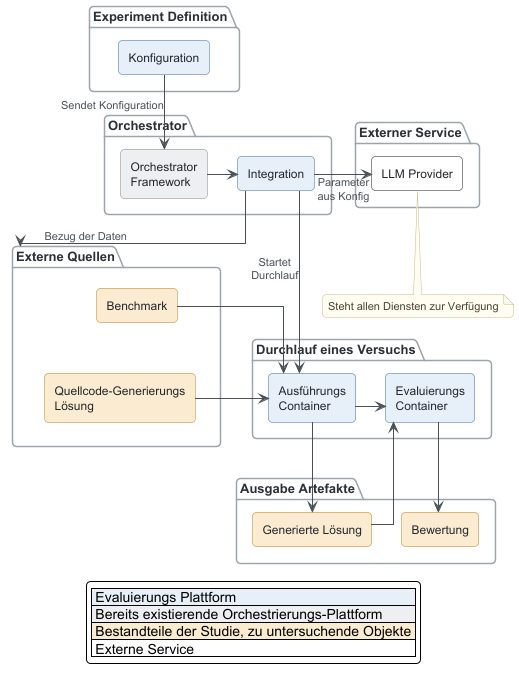
\includegraphics[width=1\linewidth]{images/rough_architecture.png}
    \caption{Architektur der Evaluierungs Plattform}
    \label{fig:rough_architecture}
\end{figure}

Zentraler Bedeutung ist hier zunächst die eigene Integration, welche Verantwortlich für die Nutzung von Quellcodelösung und Benchmark ist. Durch sie muss dem etablierten Orchestrator Framework ermöglicht werden dedizierte Container für die Durchführung von Experimenten zu erstellen. Diese Container führen dann die Generierung und die Evaluierung von Lösungen aus.

Sowohl die generierte Lösung als auch die Bewertung des Benchmarks müssen außgegeben werden. Um den Anforderungen gerecht zu werden, müssen die ausgegebenen Artefakte aber auch die Konfiguration des Experiments und alle relevanten Parameter beinhalten, denn nur so ist es möglich diesen Prozess später nachzuverfolgen.

\subsection{Annahmen und Alternativen (?)}

\todo[inline]{Bei Alternativen wirklich überlegen ob das hier Halt hat, ist nur erstmal eine Idee in Hinsicht auf Kontrollfrage 16. Deckt sich evtl schon etwas mit subsection zu Abgrenzung.}

\controlquestions{
Für dieses Kapitel in einer Abschlussarbeit ist es wichtig, dass sowohl die Ziele und Anforderungen an die Lösung sauber hergeleitet als auch ein durchdachtes Konzept zur Erfüllung dieser Anforderungen präsentiert.
Dieses Kapitel baut in der Regel direkt auf der Analyse des Problems oder des Status quo auf und legt die Grundlage für die spätere Umsetzung.
\begin{enumerate}
    \item Wurden die Anforderungen aus den Forschungsfragen (siehe Kapitel \ref{ch:Motivation und Problemdefinition}) hergeleitet?
    \item Ist der Zusammenhang zwischen Anforderungen und übergeordneten Zielen/Forschungsfragen nachvollziehbar?    
    \item Gibt es eine nachvollziehbare Verbindung zu den Erkenntnissen aus der Analyse der verwandten Arbeiten (vgl.~Kapitel \ref{ch:Verwandte Arbeiten})?
    \item Sind funktionale Anforderungen angemessen berücksichtigt sowie eindeutig und vollständig formuliert?
    \item Sind nicht-funktionale Anforderungen eindeutig und vollständig formuliert?
    \item Sind die Anforderungen überprüfbar/testbar formuliert?
    \item Sind externe Abhängigkeiten oder Rahmenbedingungen (z.\,B. Plattformen, Zielgruppen, Datenquellen) eindeutig und nachvollziehbar dargestellt?
    \item Ist klar, welches Ziel das Konzept verfolgt?
    \item Ist das vorgeschlagene Konzept logisch und konsistent aufgebaut?
    \item Ist die Systemarchitektur bzw. das technische Design verständlich und nachvollziehbar beschrieben?
    \item Wurden Entscheidungen aus den Anforderungen oder aus der Literatur (vgl.~Kapitel \ref{ch:Verwandte Arbeiten}) hergeleitet?
    \item Wurden Annahmen getroffen oder Einschränkungen akzeptiert – und sind diese offengelegt und diskutiert?
    \item Ist ersichtlich, auf welchen Annahmen das Konzept basiert?
    \item Wird erklärt, wie das Konzept die zuvor definierten Anforderungen erfüllt?
    \item Gibt es Abbildungen (z.\,B.~UML-Diagramme, Systemübersichten, Prozessmodelle), die die Umsetzung visualisieren?
    \item Wurden Alternativen zum Konzept dargestellt, die in Betracht gezogen oder bewusst ausgeschlossen wurden?
    \item Ist das Konzept unabhängig von der konkreten Umsetzung (also ohne den Quellcode) verständlich?
    \item Ist das Konzept so (nachhaltig) formuliert, dass es auch anders umgesetzt/implementiert werden könnte?
\end{enumerate}
}